\documentclass[12pt,a4paper]{article}
\usepackage{amsmath, amssymb, geometry, booktabs, xcolor, hyperref,
            listings, pgfplots, tcolorbox, enumitem, fancyhdr, tikz, array}
\usepgfplotslibrary{fillbetween}
\geometry{margin=2.5cm}
\pgfplotsset{compat=1.18}
\tcbuselibrary{skins, breakable}

% Define custom environments
\newtcolorbox{curiositybox}[1]{colback=yellow!10, colframe=orange!80, title=#1, breakable}
\newtcolorbox{infobox}[1]{colback=blue!5, colframe=blue!60, title=#1, breakable}
\newtcolorbox{mistakebox}[1]{colback=red!5, colframe=red!60, title=#1, breakable}
\newtcolorbox{learnbox}[1]{colback=green!5, colframe=green!60, title=#1, breakable}

% Header and Footer
\pagestyle{fancy}
\fancyhf{}
\lhead{Diagonalization and Similarity Transformation}
\rhead{Unit 2 -- LAC}
\cfoot{\thepage}

% Document Title Setup
\title{\textbf{Diagonalization and Similarity Transformation} \\ \large Unit 2 -- Eigenvalues, Eigenvectors, Diagonalization and Quadratic Forms}
\author{Department of Mathematics}
\date{\today}

\begin{document}
\maketitle
\tableofcontents
\newpage

%% ============================================================
%% SECTION 1: REAL-WORLD ENGINEERING HOOK
%% ============================================================
\section{Real-World Engineering Hook}

\begin{curiositybox}{Why Should an Engineer Care?}
\textbf{Scenario 1 --- Multi-DOF Vibration Decoupling.}
In the structural analysis of a five-storey building during an earthquake, the equations of motion form a coupled system
\[
  M\ddot{\mathbf{x}} + K\mathbf{x} = \mathbf{f}(t),
\]
where $M$ and $K$ are $5\times 5$ mass and stiffness matrices.
Solving five mutually coupled ODEs simultaneously is brutal.
Diagonalization via the modal matrix $P$ transforms this into five \emph{independent} single-DOF oscillators --- each solved trivially.
Without diagonalization, every floor's motion contaminates every other floor's equation.

\textbf{Scenario 2 --- Principal Component Analysis (PCA) in Data Compression.}
A face-recognition system stores $10\,000$-pixel images.
The covariance matrix of the image dataset is symmetric and positive semi-definite.
Orthogonal diagonalization ($A = Q\Lambda Q^{T}$) extracts orthogonal ``principal axes'' (eigenvectors) so that 95\% of the information lives in the top 50 components instead of 10\,000 --- a 200$\times$ compression with negligible quality loss.

\textbf{Scenario 3 --- Markov Chains and Population Dynamics.}
A wildlife biologist models annual transitions among juvenile, sub-adult, and adult populations with a $3\times 3$ transition matrix $A$.
Predicting the population after 40 years requires $A^{40}$.
Direct multiplication is 39 matrix products; via diagonalization $A^{40} = P D^{40} P^{-1}$, where $D^{40}$ is computed by simply raising three scalar eigenvalues to the 40th power --- three multiplications instead of thousands.
\end{curiositybox}

%% ============================================================
%% SECTION 2: WHY THIS TOPIC EXISTS
%% ============================================================
\section{Why This Topic Exists}

\begin{center}
\begin{tabular}{@{}p{3.5cm}p{5cm}p{6cm}@{}}
\toprule
\textbf{Sub-Topic} & \textbf{Core Idea} & \textbf{Engineering Consequence} \\
\midrule
Similarity Transformation & $B = P^{-1}AP$ preserves eigenvalues, trace, determinant & Coordinate change in vibration analysis; same physics, simpler mathematics \\
\addlinespace
Diagonalizability Condition & $n$ linearly independent eigenvectors exist iff geometric multiplicity $=$ algebraic multiplicity & Determines whether modal decomposition of a structural system is possible \\
\addlinespace
Diagonalization Procedure & Form $P$ from eigenvectors; compute $D = P^{-1}AP$ & Decouples ODEs in control systems; enables closed-form solutions \\
\addlinespace
Powers of Matrix & $A^{n} = P D^{n} P^{-1}$; $D^{n}$ trivial to compute & Long-horizon Markov chain prediction; iterated map simulation in robotics \\
\addlinespace
Orthogonal Diagonalization & Symmetric $A = Q\Lambda Q^{T}$ with orthonormal $Q$ & PCA, finite-element stress analysis, quadratic form classification \\
\bottomrule
\end{tabular}
\end{center}

\begin{learnbox}{Core Learning Objectives}
After studying this topic you will be able to:
\begin{enumerate}[leftmargin=*]
  \item Define similarity transformation and state invariant properties under it.
  \item Determine whether a matrix is diagonalizable and explain why.
  \item Execute the full diagonalization procedure for $2\times 2$ and $3\times 3$ matrices.
  \item Compute $A^{n}$ efficiently using $A^{n} = PD^{n}P^{-1}$.
  \item Orthogonally diagonalize real symmetric matrices using orthonormal eigenvectors.
\end{enumerate}
\end{learnbox}

%% ============================================================
%% SECTION 3: INTUITION + DEFINITIONS (EXACTLY 5 SUBSECTIONS)
%% ============================================================
\section{Intuition and Mathematical Definitions}

\subsection{Similarity Transformation}

Think of two mathematicians describing the \emph{same} linear map but using different coordinate systems.
One uses the standard basis $\{e_1, e_2\}$; the other uses a rotated basis.
The matrices they write down look different, yet they encode the identical transformation.
A similarity transformation is precisely this change-of-basis operation: $B = P^{-1}AP$.
Because the underlying transformation is unchanged, fundamental invariants --- eigenvalues, trace, determinant, rank --- are shared by $A$ and $B$.

\begin{infobox}{Similarity Transformation --- Formal Definitions}
\textbf{Definition.}
Two $n\times n$ matrices $A$ and $B$ are \emph{similar} if there exists an invertible matrix $P$ such that
\[
  B = P^{-1}AP.
\]
$P$ is called the \emph{similarity (transition) matrix}.

\textbf{Key Invariants Under Similarity.}
If $B = P^{-1}AP$, then:
\begin{itemize}[leftmargin=*]
  \item $\det(B) = \det(A)$
  \item $\operatorname{tr}(B) = \operatorname{tr}(A)$
  \item $\operatorname{rank}(B) = \operatorname{rank}(A)$
  \item $A$ and $B$ have the \emph{same characteristic polynomial}, hence the same eigenvalues with the same algebraic multiplicities.
\end{itemize}

\textbf{Proof sketch (eigenvalue preservation).}
\begin{align*}
  \det(B - \lambda I) &= \det(P^{-1}AP - \lambda I)\\
                      &= \det(P^{-1}(A-\lambda I)P)\\
                      &= \det(P^{-1})\det(A-\lambda I)\det(P)\\
                      &= \det(A-\lambda I).
\end{align*}

\textbf{Similarity is an equivalence relation:}
reflexive ($A = I^{-1}AI$), symmetric (if $B=P^{-1}AP$ then $A=PBP^{-1}$), transitive.
\end{infobox}

\textbf{Worked Example 1.1 --- Verifying Shared Eigenvalues Under Similarity.}

Let
\[
  A = \begin{pmatrix} 4 & 1 \\ 2 & 3 \end{pmatrix}, \qquad
  P = \begin{pmatrix} 1 & 1 \\ 2 & -1 \end{pmatrix}.
\]
\textbf{Step 1.} Compute $\det(P) = (1)(-1)-(1)(2) = -1-2 = -3 \neq 0$. So $P$ is invertible.

\textbf{Step 2.} Compute $P^{-1}$.
\[
  P^{-1} = \frac{1}{-3}\begin{pmatrix} -1 & -1 \\ -2 & 1 \end{pmatrix}
          = \begin{pmatrix} 1/3 & 1/3 \\ 2/3 & -1/3 \end{pmatrix}.
\]

\textbf{Step 3.} Compute $B = P^{-1}AP$.
\[
  AP = \begin{pmatrix} 4 & 1 \\ 2 & 3 \end{pmatrix}\begin{pmatrix} 1 & 1 \\ 2 & -1 \end{pmatrix}
     = \begin{pmatrix} 4\cdot1+1\cdot2 & 4\cdot1+1\cdot(-1) \\ 2\cdot1+3\cdot2 & 2\cdot1+3\cdot(-1) \end{pmatrix}
     = \begin{pmatrix} 6 & 3 \\ 8 & -1 \end{pmatrix}.
\]
\[
  B = P^{-1}(AP) = \begin{pmatrix} 1/3 & 1/3 \\ 2/3 & -1/3 \end{pmatrix}\begin{pmatrix} 6 & 3 \\ 8 & -1 \end{pmatrix}
    = \begin{pmatrix} 6/3+8/3 & 3/3-1/3 \\ 12/3-8/3 & 6/3+1/3 \end{pmatrix}
    = \begin{pmatrix} 14/3 & 2/3 \\ 4/3 & 7/3 \end{pmatrix}.
\]

\textbf{Step 4.} Check traces: $\operatorname{tr}(A) = 4+3 = 7$; $\operatorname{tr}(B) = 14/3+7/3 = 21/3 = 7$. \checkmark \\
Check determinants: $\det(A) = 12-2 = 10$; $\det(B) = (14/3)(7/3)-(2/3)(4/3) = 98/9-8/9 = 90/9 = 10$. \checkmark

Both matrices share $\operatorname{tr}=7$ and $\det=10$, confirming the characteristic polynomial $\lambda^2 - 7\lambda + 10 = 0$ and eigenvalues $\lambda = 5, 2$ for both.

% ---

\subsection{Diagonalizability Condition}

Imagine trying to build a basis for $\mathbb{R}^n$ entirely out of eigenvectors.
If you succeed --- if $n$ independent eigenvectors exist --- then you can represent $A$ in that eigenvector basis, and the matrix looks diagonal.
If even one direction has ``too few'' eigenvectors (geometric multiplicity less than algebraic multiplicity for some eigenvalue), the basis fails and diagonalization is impossible.

\begin{infobox}{Diagonalizability Condition --- Formal Definitions}
\textbf{Definition (Diagonalizable).}
An $n\times n$ matrix $A$ is \emph{diagonalizable} over $\mathbb{R}$ if there exists an invertible $P$ such that $P^{-1}AP = D$ where $D$ is diagonal.

\textbf{Fundamental Theorem.}
$A$ is diagonalizable \emph{if and only if} $A$ has $n$ linearly independent eigenvectors (i.e., they form a basis of $\mathbb{R}^n$).

\textbf{Multiplicity Criterion.}
For each eigenvalue $\lambda_i$:
\[
  \text{geometric multiplicity}(\lambda_i) \;=\; \dim(\ker(A - \lambda_i I))
\]
\[
  \text{algebraic multiplicity}(\lambda_i) \;=\; \text{exponent of } (\lambda - \lambda_i) \text{ in } \det(A-\lambda I).
\]
$A$ is diagonalizable $\Longleftrightarrow$ geometric multiplicity $=$ algebraic multiplicity for \emph{every} eigenvalue.

\textbf{Sufficient (not necessary) condition.}
If $A$ has $n$ \emph{distinct} eigenvalues, it is automatically diagonalizable.

\textbf{Defective matrix.}
If geometric multiplicity $<$ algebraic multiplicity for some $\lambda_i$, $A$ is called \emph{defective} and cannot be diagonalized (only Jordan form is possible).
\end{infobox}

\textbf{Worked Example 2.1 --- Diagonalizable vs. Non-Diagonalizable.}

\medskip
\textit{Case A: Diagonalizable.} Let $A = \begin{pmatrix} 3 & 1 \\ 0 & 5 \end{pmatrix}$.

Characteristic polynomial: $\det(A-\lambda I) = (3-\lambda)(5-\lambda) = 0 \Rightarrow \lambda_1 = 3,\, \lambda_2 = 5$.
Two distinct eigenvalues $\Rightarrow$ automatically diagonalizable.

For $\lambda_1 = 3$: $(A-3I)\mathbf{v} = \mathbf{0} \Rightarrow \begin{pmatrix}0&1\\0&2\end{pmatrix}\mathbf{v}=\mathbf{0} \Rightarrow \mathbf{v}_1 = \begin{pmatrix}1\\0\end{pmatrix}$.

For $\lambda_2 = 5$: $(A-5I)\mathbf{v} = \mathbf{0} \Rightarrow \begin{pmatrix}-2&1\\0&0\end{pmatrix}\mathbf{v}=\mathbf{0} \Rightarrow \mathbf{v}_2 = \begin{pmatrix}1\\2\end{pmatrix}$.

Two independent eigenvectors confirmed: diagonalizable.

\medskip
\textit{Case B: Non-Diagonalizable.} Let $B = \begin{pmatrix} 4 & 1 \\ 0 & 4 \end{pmatrix}$.

Characteristic polynomial: $(4-\lambda)^2 = 0 \Rightarrow \lambda = 4$ with algebraic multiplicity 2.

Eigenspace: $(B-4I)\mathbf{v} = \begin{pmatrix}0&1\\0&0\end{pmatrix}\mathbf{v} = \mathbf{0} \Rightarrow v_2 = 0$, $v_1$ free. Eigenvectors: $\mathbf{v} = t\begin{pmatrix}1\\0\end{pmatrix}$.

Geometric multiplicity $= 1 < 2 =$ algebraic multiplicity. Therefore $B$ is \emph{defective} and \textbf{not diagonalizable}.

% ---

\subsection{Diagonalization Procedure}

The procedure is like solving a jigsaw puzzle with three pieces: eigenvalues (from the characteristic equation), eigenvectors (from null-space computations), and the final assembly (form $P$, compute $D = P^{-1}AP$).
Once you have assembled $P$ correctly, the diagonal entries of $D$ are exactly the eigenvalues in the order the eigenvectors were placed as columns of $P$.

\begin{infobox}{Diagonalization Procedure --- Step-by-Step Algorithm}
Given an $n\times n$ matrix $A$:

\textbf{Step 1.} Find all eigenvalues by solving $\det(A - \lambda I) = 0$.

\textbf{Step 2.} For each eigenvalue $\lambda_i$, find a basis for $\ker(A - \lambda_i I)$ by row-reducing $A - \lambda_i I$.

\textbf{Step 3.} Check: total number of linearly independent eigenvectors $= n$? If yes, proceed; otherwise $A$ is not diagonalizable.

\textbf{Step 4.} Form the \emph{modal matrix} $P$ by placing the eigenvectors as columns in any consistent order:
\[
  P = \begin{pmatrix} \mathbf{v}_1 & \mathbf{v}_2 & \cdots & \mathbf{v}_n \end{pmatrix}.
\]

\textbf{Step 5.} The diagonal matrix is:
\[
  D = P^{-1}AP = \begin{pmatrix} \lambda_1 & 0 & \cdots & 0 \\ 0 & \lambda_2 & \cdots & 0 \\ \vdots & & \ddots & \vdots \\ 0 & 0 & \cdots & \lambda_n \end{pmatrix},
\]
where $\lambda_i$ in position $(i,i)$ corresponds to eigenvector in column $i$ of $P$.

\textbf{Verification:} Confirm $AP = PD$ (avoids inverting $P$ explicitly for the check).
\end{infobox}

\textbf{Worked Example 3.1 --- Full $3\times 3$ Diagonalization.}

Let
\[
  A = \begin{pmatrix} 2 & 1 & 0 \\ 0 & 3 & 0 \\ 0 & 1 & 2 \end{pmatrix}.
\]

\textbf{Step 1: Eigenvalues.}
\[
  \det(A-\lambda I) = \det\begin{pmatrix}2-\lambda&1&0\\0&3-\lambda&0\\0&1&2-\lambda\end{pmatrix}.
\]
Expanding along column 3:
\[
  = (2-\lambda)\,\det\begin{pmatrix}2-\lambda&1\\0&3-\lambda\end{pmatrix}
  = (2-\lambda)\bigl[(2-\lambda)(3-\lambda) - 0\bigr]
  = (2-\lambda)^2(3-\lambda).
\]
Eigenvalues: $\lambda_1 = 2$ (algebraic multiplicity 2), $\lambda_2 = 3$ (algebraic multiplicity 1).

\textbf{Step 2: Eigenvectors.}

For $\lambda = 2$: $A - 2I = \begin{pmatrix}0&1&0\\0&1&0\\0&1&0\end{pmatrix}$. Row reduce: one independent equation $v_2 = 0$; $v_1, v_3$ free.
Two independent eigenvectors:
\[
  \mathbf{v}_1 = \begin{pmatrix}1\\0\\0\end{pmatrix}, \quad \mathbf{v}_2 = \begin{pmatrix}0\\0\\1\end{pmatrix}.
\]
Geometric multiplicity $= 2 =$ algebraic multiplicity. \checkmark

For $\lambda = 3$: $A - 3I = \begin{pmatrix}-1&1&0\\0&0&0\\0&1&-1\end{pmatrix}$.
Row 1: $-v_1+v_2=0 \Rightarrow v_1=v_2$. Row 3: $v_2=v_3$. Set $v_2=1$: $\mathbf{v}_3 = \begin{pmatrix}1\\1\\1\end{pmatrix}$.

\textbf{Step 3: Diagonalizability.} 3 independent eigenvectors for a $3\times 3$ matrix. \checkmark

\textbf{Step 4: Form $P$.}
\[
  P = \begin{pmatrix}1&0&1\\0&0&1\\0&1&1\end{pmatrix}.
\]

\textbf{Step 5: Verify $AP = PD$ where $D = \operatorname{diag}(2,2,3)$.}
\[
  AP = \begin{pmatrix}2&1&0\\0&3&0\\0&1&2\end{pmatrix}\begin{pmatrix}1&0&1\\0&0&1\\0&1&1\end{pmatrix}
     = \begin{pmatrix}2&1&3\\0&0&3\\0&1&3\end{pmatrix}.
\]
\[
  PD = \begin{pmatrix}1&0&1\\0&0&1\\0&1&1\end{pmatrix}\begin{pmatrix}2&0&0\\0&2&0\\0&0&3\end{pmatrix}
     = \begin{pmatrix}2&0&3\\0&0&3\\0&2&3\end{pmatrix}.
\]
Hmm, column 2: $AP$ gives $(1, 0, 1)^T$ and $PD$ gives $(0,0,2)^T$. These differ because $\mathbf{v}_2 = (0,0,1)^T$ is the second eigenvector for $\lambda=2$, let us re-verify.

$A\mathbf{v}_2 = \begin{pmatrix}2&1&0\\0&3&0\\0&1&2\end{pmatrix}\begin{pmatrix}0\\0\\1\end{pmatrix} = \begin{pmatrix}0\\0\\2\end{pmatrix} = 2\begin{pmatrix}0\\0\\1\end{pmatrix}$. \checkmark

$A\mathbf{v}_1 = \begin{pmatrix}2&1&0\\0&3&0\\0&1&2\end{pmatrix}\begin{pmatrix}1\\0\\0\end{pmatrix} = \begin{pmatrix}2\\0\\0\end{pmatrix} = 2\begin{pmatrix}1\\0\\0\end{pmatrix}$. \checkmark

$A\mathbf{v}_3 = \begin{pmatrix}2&1&0\\0&3&0\\0&1&2\end{pmatrix}\begin{pmatrix}1\\1\\1\end{pmatrix} = \begin{pmatrix}3\\3\\3\end{pmatrix} = 3\begin{pmatrix}1\\1\\1\end{pmatrix}$. \checkmark

All eigenvector-eigenvalue relations verified; $D = \operatorname{diag}(2,2,3)$.

% ---

\subsection{Powers of Matrix via Diagonalization}

Raising a matrix to a high power by repeated multiplication is exhausting.
Diagonalization turns this into a one-line formula because powers of a diagonal matrix are trivial: just raise each diagonal entry to the required power.
This is one of the most practically powerful results in all of applied linear algebra.

\begin{infobox}{Matrix Powers via Diagonalization}
\textbf{Formula.}
If $A = PDP^{-1}$ (with $D = \operatorname{diag}(\lambda_1,\ldots,\lambda_n)$), then for any positive integer $k$:
\[
  A^{k} = P D^{k} P^{-1}, \quad \text{where } D^{k} = \operatorname{diag}(\lambda_1^k, \lambda_2^k, \ldots, \lambda_n^k).
\]

\textbf{Derivation.}
\begin{align*}
  A^{2} &= (PDP^{-1})(PDP^{-1}) = PD(P^{-1}P)DP^{-1} = PD^{2}P^{-1},\\
  A^{k} &= P\underbrace{D\cdot D\cdots D}_{k}P^{-1} = PD^{k}P^{-1}.
\end{align*}

\textbf{Extension.}
For $k = 0$: $A^0 = PIP^{-1} = I$. For negative $k$ (if $A$ invertible): $A^{-k} = PD^{-k}P^{-1}$.

\textbf{Computational saving.}
Direct computation of $A^{k}$ requires $O(kn^3)$ multiplications.
Via diagonalization: $O(n^3)$ once to find $P$ and $P^{-1}$, then $O(n)$ to compute $\lambda_i^k$. For large $k$, the saving is enormous.
\end{infobox}

\textbf{Worked Example 4.1 --- Computing $A^5$ via Diagonalization.}

Let
\[
  A = \begin{pmatrix} 1 & 2 \\ 0 & 3 \end{pmatrix}.
\]

\textbf{Step 1: Eigenvalues.}
$\det(A - \lambda I) = (1-\lambda)(3-\lambda) = 0 \Rightarrow \lambda_1 = 1,\; \lambda_2 = 3$.

\textbf{Step 2: Eigenvectors.}

$\lambda_1 = 1$: $(A-I)\mathbf{v} = \begin{pmatrix}0&2\\0&2\end{pmatrix}\mathbf{v} = \mathbf{0} \Rightarrow v_2 = 0$. So $\mathbf{v}_1 = \begin{pmatrix}1\\0\end{pmatrix}$.

$\lambda_2 = 3$: $(A-3I)\mathbf{v} = \begin{pmatrix}-2&2\\0&0\end{pmatrix}\mathbf{v} = \mathbf{0} \Rightarrow v_1 = v_2$. So $\mathbf{v}_2 = \begin{pmatrix}1\\1\end{pmatrix}$.

\textbf{Step 3: Form $P$ and $D$.}
\[
  P = \begin{pmatrix}1&1\\0&1\end{pmatrix}, \qquad D = \begin{pmatrix}1&0\\0&3\end{pmatrix}.
\]

\textbf{Step 4: Compute $P^{-1}$.}
$\det(P) = 1$, so $P^{-1} = \begin{pmatrix}1&-1\\0&1\end{pmatrix}$.

\textbf{Step 5: Compute $D^5$.}
\[
  D^5 = \begin{pmatrix}1^5&0\\0&3^5\end{pmatrix} = \begin{pmatrix}1&0\\0&243\end{pmatrix}.
\]

\textbf{Step 6: Compute $A^5 = PD^5P^{-1}$.}
\[
  PD^5 = \begin{pmatrix}1&1\\0&1\end{pmatrix}\begin{pmatrix}1&0\\0&243\end{pmatrix}
       = \begin{pmatrix}1&243\\0&243\end{pmatrix}.
\]
\[
  A^5 = (PD^5)P^{-1} = \begin{pmatrix}1&243\\0&243\end{pmatrix}\begin{pmatrix}1&-1\\0&1\end{pmatrix}
       = \begin{pmatrix}1\cdot1+243\cdot0 & 1\cdot(-1)+243\cdot1 \\ 0\cdot1+243\cdot0 & 0\cdot(-1)+243\cdot1\end{pmatrix}
       = \begin{pmatrix}1&242\\0&243\end{pmatrix}.
\]

\textbf{Verification (checking $(1,2)$ entry directly):}
$A^2 = \begin{pmatrix}1&8\\0&9\end{pmatrix}$, $A^3 = \begin{pmatrix}1&26\\0&27\end{pmatrix}$, $A^4 = \begin{pmatrix}1&80\\0&81\end{pmatrix}$, $A^5 = \begin{pmatrix}1&242\\0&243\end{pmatrix}$. \checkmark

% ---

\subsection{Orthogonal Diagonalization}

Real symmetric matrices are special: their eigenvectors for \emph{distinct} eigenvalues are automatically orthogonal to each other.
This means we can form an orthonormal basis from eigenvectors and use it as the columns of $Q$.
The result $A = Q\Lambda Q^T$ is not just a similarity transformation --- it is an \emph{isometry-preserving} decomposition that reveals the principal axes of the quadratic form $\mathbf{x}^T A \mathbf{x}$.

\begin{infobox}{Orthogonal Diagonalization --- Definitions and Theorems}
\textbf{Definition (Orthogonally Diagonalizable).}
A real $n\times n$ matrix $A$ is orthogonally diagonalizable if there exists a real \emph{orthogonal} matrix $Q$ ($Q^T Q = I$, so $Q^{-1} = Q^T$) such that
\[
  Q^T A Q = \Lambda = \operatorname{diag}(\lambda_1, \ldots, \lambda_n).
\]
Equivalently, $A = Q\Lambda Q^T$.

\textbf{Spectral Theorem.}
A real matrix $A$ is orthogonally diagonalizable \emph{if and only if} $A$ is \emph{symmetric} ($A = A^T$).

\textbf{Orthogonality of eigenvectors.}
If $A = A^T$ and $A\mathbf{v} = \lambda\mathbf{v}$, $A\mathbf{w} = \mu\mathbf{w}$ with $\lambda \neq \mu$, then $\mathbf{v} \cdot \mathbf{w} = 0$.

\textbf{Procedure for orthogonal diagonalization:}
\begin{enumerate}[leftmargin=*]
  \item Find all eigenvalues of the symmetric matrix $A$.
  \item For each eigenvalue, find the eigenspace basis.
  \item If an eigenvalue has algebraic multiplicity $> 1$, apply Gram--Schmidt to the eigenspace basis to get orthonormal vectors.
  \item Normalize all eigenvectors: $\hat{\mathbf{q}}_i = \mathbf{v}_i / \|\mathbf{v}_i\|$.
  \item Form $Q = \begin{pmatrix}\hat{\mathbf{q}}_1 & \hat{\mathbf{q}}_2 & \cdots & \hat{\mathbf{q}}_n\end{pmatrix}$.
  \item Then $Q^T A Q = \Lambda$.
\end{enumerate}

\textbf{Spectral decomposition:}
\[
  A = \lambda_1 \hat{\mathbf{q}}_1\hat{\mathbf{q}}_1^T + \lambda_2 \hat{\mathbf{q}}_2\hat{\mathbf{q}}_2^T + \cdots + \lambda_n \hat{\mathbf{q}}_n\hat{\mathbf{q}}_n^T.
\]
\end{infobox}

\textbf{Worked Example 5.1 --- Orthogonal Diagonalization of a $2\times 2$ Symmetric Matrix.}

Let
\[
  A = \begin{pmatrix} 5 & 2 \\ 2 & 2 \end{pmatrix}.
\]
Note $A = A^T$, so orthogonal diagonalization is guaranteed.

\textbf{Step 1: Eigenvalues.}
\[
  \det(A-\lambda I) = (5-\lambda)(2-\lambda) - 4 = \lambda^2 - 7\lambda + 6 = (\lambda-1)(\lambda-6) = 0.
\]
$\lambda_1 = 1$, $\lambda_2 = 6$.

\textbf{Step 2: Eigenvectors.}

$\lambda_1 = 1$: $(A-I)\mathbf{v} = \begin{pmatrix}4&2\\2&1\end{pmatrix}\mathbf{v} = \mathbf{0}$. Row 1: $4v_1+2v_2=0 \Rightarrow v_2 = -2v_1$. Set $v_1=1$: $\mathbf{v}_1 = \begin{pmatrix}1\\-2\end{pmatrix}$.

$\lambda_2 = 6$: $(A-6I)\mathbf{v} = \begin{pmatrix}-1&2\\2&-4\end{pmatrix}\mathbf{v} = \mathbf{0}$. Row 1: $-v_1+2v_2=0 \Rightarrow v_1=2v_2$. Set $v_2=1$: $\mathbf{v}_2 = \begin{pmatrix}2\\1\end{pmatrix}$.

\textbf{Check orthogonality:} $\mathbf{v}_1 \cdot \mathbf{v}_2 = (1)(2)+(-2)(1) = 2-2 = 0$. \checkmark

\textbf{Step 3: Normalize.}
$\|\mathbf{v}_1\| = \sqrt{1+4} = \sqrt{5}$, so $\hat{\mathbf{q}}_1 = \dfrac{1}{\sqrt{5}}\begin{pmatrix}1\\-2\end{pmatrix}$.

$\|\mathbf{v}_2\| = \sqrt{4+1} = \sqrt{5}$, so $\hat{\mathbf{q}}_2 = \dfrac{1}{\sqrt{5}}\begin{pmatrix}2\\1\end{pmatrix}$.

\textbf{Step 4: Form $Q$.}
\[
  Q = \dfrac{1}{\sqrt{5}}\begin{pmatrix}1&2\\-2&1\end{pmatrix}, \qquad \Lambda = \begin{pmatrix}1&0\\0&6\end{pmatrix}.
\]

\textbf{Verify $Q^TAQ = \Lambda$:}
$Q^T = \dfrac{1}{\sqrt{5}}\begin{pmatrix}1&-2\\2&1\end{pmatrix}$.
\[
  AQ = \begin{pmatrix}5&2\\2&2\end{pmatrix}\cdot\dfrac{1}{\sqrt{5}}\begin{pmatrix}1&2\\-2&1\end{pmatrix}
     = \dfrac{1}{\sqrt{5}}\begin{pmatrix}5-4&10+2\\2-4&4+2\end{pmatrix}
     = \dfrac{1}{\sqrt{5}}\begin{pmatrix}1&12\\-2&6\end{pmatrix}.
\]
\[
  Q^T(AQ) = \dfrac{1}{\sqrt{5}}\begin{pmatrix}1&-2\\2&1\end{pmatrix}\cdot\dfrac{1}{\sqrt{5}}\begin{pmatrix}1&12\\-2&6\end{pmatrix}
           = \dfrac{1}{5}\begin{pmatrix}1+4&12-12\\2-2&24+6\end{pmatrix}
           = \dfrac{1}{5}\begin{pmatrix}5&0\\0&30\end{pmatrix}
           = \begin{pmatrix}1&0\\0&6\end{pmatrix} = \Lambda. \checkmark
\]

%% ============================================================
%% SECTION 4: VISUAL ARTIFACTS
%% ============================================================
\section{Visual Artifacts and Geometric Interpretation}

\subsection*{Diagram 1: Similarity Transformation Flow $A \to P^{-1}AP = D$}

\begin{center}
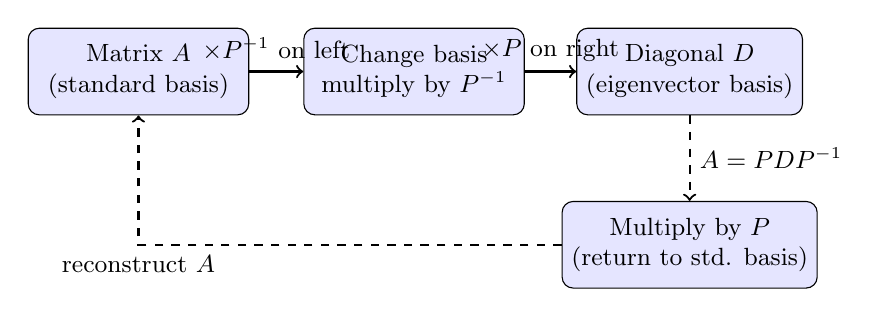
\begin{tikzpicture}[node distance=3.5cm, auto,
  box/.style={draw, fill=blue!10, rounded corners, minimum width=2.8cm, minimum height=1.1cm, align=center, font=\small}]
  \node[box] (A) {Matrix $A$\\(standard basis)};
  \node[box, right of=A] (coord) {Change basis\\multiply by $P^{-1}$};
  \node[box, right of=coord] (D) {Diagonal $D$\\(eigenvector basis)};
  \node[box, below of=D, node distance=2.2cm] (back) {Multiply by $P$\\(return to std. basis)};
  \draw[->, thick] (A) -- node[above]{\small $\times P^{-1}$ on left} (coord);
  \draw[->, thick] (coord) -- node[above]{\small $\times P$ on right} (D);
  \draw[->, thick, dashed] (D) -- node[right]{\small $A = PDP^{-1}$} (back);
  \draw[->, thick, dashed] (back) -| node[below]{\small reconstruct $A$} (A);
\end{tikzpicture}
\end{center}

\subsection*{Diagram 2: Orthogonal Eigenvectors of a Symmetric Matrix}

\begin{center}
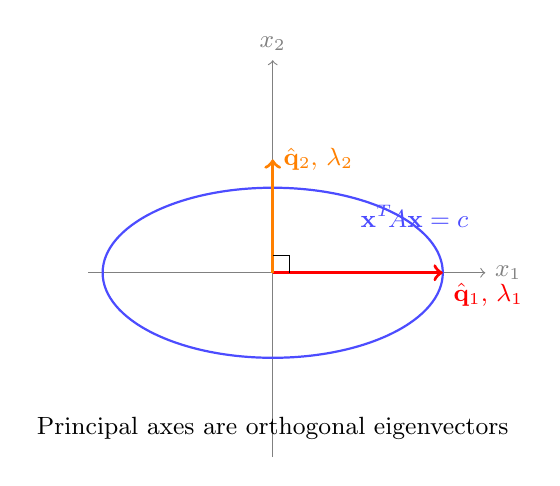
\begin{tikzpicture}[scale=1.8]
  % Standard axes
  \draw[->, gray, thin] (-1.3,0) -- (1.5,0) node[right]{\small $x_1$};
  \draw[->, gray, thin] (0,-1.3) -- (0,1.5) node[above]{\small $x_2$};
  % Ellipse representing level curve of x^T A x = const
  \draw[blue!70, thick] (0,0) ellipse (1.2cm and 0.6cm);
  \node[blue!70] at (1.0, 0.4) {\small $\mathbf{x}^T\!A\mathbf{x}=c$};
  % Eigenvector 1 (major axis direction)
  \draw[->, very thick, red] (0,0) -- (1.2,0) node[below right]{\small $\hat{\mathbf{q}}_1$, $\lambda_1$};
  % Eigenvector 2 (minor axis direction)
  \draw[->, very thick, orange] (0,0) -- (0,0.8) node[right]{\small $\hat{\mathbf{q}}_2$, $\lambda_2$};
  % Right angle marker
  \draw (0.12,0) -- (0.12,0.12) -- (0,0.12);
  \node at (0,-1.1) {\small Principal axes are orthogonal eigenvectors};
\end{tikzpicture}
\end{center}

\subsection*{Diagram 3: Matrix Power Computation via Diagonalization}

\begin{center}
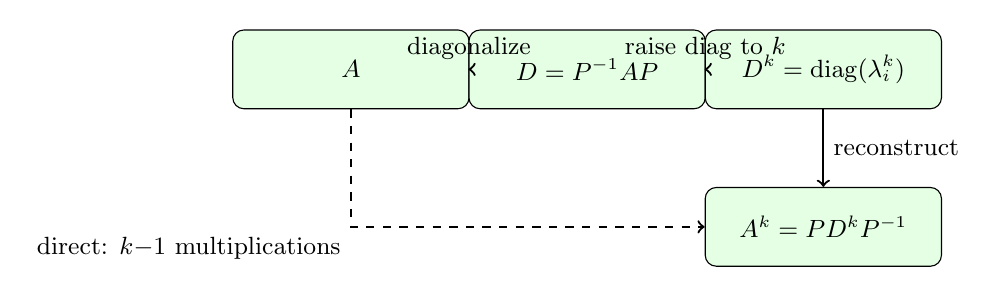
\begin{tikzpicture}[node distance=3.0cm, auto,
  box/.style={draw, fill=green!10, rounded corners, minimum width=3.0cm, minimum height=1.0cm, align=center, font=\small}]
  \node[box] (A) {$A$};
  \node[box, right of=A] (D) {$D = P^{-1}AP$};
  \node[box, right of=D] (Dk) {$D^k = \operatorname{diag}(\lambda_i^k)$};
  \node[box, below of=Dk, node distance=2.0cm] (Ak) {$A^k = PD^k P^{-1}$};
  \draw[->, thick] (A) -- node[above]{\small diagonalize} (D);
  \draw[->, thick] (D) -- node[above]{\small raise diag to $k$} (Dk);
  \draw[->, thick] (Dk) -- node[right]{\small reconstruct} (Ak);
  \draw[->, dashed, thick] (A) |- node[below left]{\small direct: $k{-}1$ multiplications} (Ak);
\end{tikzpicture}
\end{center}

%% ============================================================
%% SECTION 5: STEP-BY-STEP ALGORITHMIC WORKFLOW
%% ============================================================
\section{Step-by-Step Algorithmic Workflow}

\begin{center}
\fbox{\parbox{0.88\textwidth}{
\textbf{DIAGONALIZATION ALGORITHM WITH DECISION TREE}

\textbf{INPUT:} $n \times n$ matrix $A$.

\medskip
\textbf{Step 1 --- Characteristic Polynomial.}
Compute $p(\lambda) = \det(A - \lambda I)$. Factor to find all eigenvalues $\lambda_1, \ldots, \lambda_k$ with algebraic multiplicities $a_1, \ldots, a_k$.

\medskip
\textbf{Step 2 --- Eigenspaces.}
For each $\lambda_i$, row-reduce $A - \lambda_i I$ to find $\ker(A-\lambda_i I)$.
Let $g_i = \dim\ker(A - \lambda_i I)$ (geometric multiplicity).

\medskip
\textbf{Step 3 --- DECISION: Is $A$ diagonalizable?}
\begin{itemize}[leftmargin=*]
  \item If $g_i = a_i$ for all $i$ \textbf{AND} $\sum g_i = n$: \textbf{YES} $\to$ proceed to Step 4.
  \item If any $g_i < a_i$: \textbf{NO} $\to$ $A$ is defective; Jordan form required. \textbf{STOP.}
\end{itemize}

\medskip
\textbf{Step 4 --- Form Modal Matrix $P$.}
Collect all eigenvectors (one basis vector per free variable per eigenspace).
Arrange as columns: $P = [\mathbf{v}_1 \mid \mathbf{v}_2 \mid \cdots \mid \mathbf{v}_n]$.

\medskip
\textbf{Step 5 --- Write $D$.}
$D = \operatorname{diag}(\lambda_{(1)}, \lambda_{(2)}, \ldots, \lambda_{(n)})$ where $\lambda_{(i)}$ is the eigenvalue for column $i$ of $P$.

\medskip
\textbf{Step 6 --- Verify (Optional but Recommended).}
Check $AP = PD$ column by column: $A\mathbf{v}_i = \lambda_{(i)}\mathbf{v}_i$.

\medskip
\textbf{Step 7 (Orthogonal variant, symmetric $A$ only).}
Apply Gram--Schmidt within each eigenspace of multiplicity $>1$.
Normalize all eigenvectors. Form orthogonal matrix $Q$; then $Q^TAQ = \Lambda$.
}}
\end{center}

%% ============================================================
%% SECTION 6: FULLY WORKED NUMERICAL EXAMPLES
%% ============================================================
\section{Fully Worked Step-by-Step Numerical Examples}

\subsection*{Example 6.1 --- Diagonalize a $2\times 2$ Matrix; Verify $D = P^{-1}AP$}

Let
\[
  A = \begin{pmatrix} 6 & -1 \\ 2 & 3 \end{pmatrix}.
\]

\textbf{Step 1: Eigenvalues.}
\[
  \det(A-\lambda I) = (6-\lambda)(3-\lambda)+2 = \lambda^2 - 9\lambda + 20 = (\lambda-4)(\lambda-5).
\]
$\lambda_1 = 4$, $\lambda_2 = 5$. Two distinct eigenvalues $\Rightarrow$ diagonalizable.

\textbf{Step 2: Eigenvectors.}

$\lambda_1=4$: $(A-4I) = \begin{pmatrix}2&-1\\2&-1\end{pmatrix}$. Row 1: $2v_1-v_2=0 \Rightarrow v_2=2v_1$. Set $v_1=1$: $\mathbf{v}_1=\begin{pmatrix}1\\2\end{pmatrix}$.

$\lambda_2=5$: $(A-5I) = \begin{pmatrix}1&-1\\2&-2\end{pmatrix}$. Row 1: $v_1-v_2=0 \Rightarrow v_1=v_2$. Set $v_1=1$: $\mathbf{v}_2=\begin{pmatrix}1\\1\end{pmatrix}$.

\textbf{Step 3: Form $P$ and $D$.}
\[
  P = \begin{pmatrix}1&1\\2&1\end{pmatrix}, \qquad D = \begin{pmatrix}4&0\\0&5\end{pmatrix}.
\]

\textbf{Step 4: Compute $P^{-1}$.}
$\det(P) = 1-2 = -1$.
\[
  P^{-1} = \frac{1}{-1}\begin{pmatrix}1&-1\\-2&1\end{pmatrix} = \begin{pmatrix}-1&1\\2&-1\end{pmatrix}.
\]

\textbf{Step 5: Verify $D = P^{-1}AP$.}
\[
  AP = \begin{pmatrix}6&-1\\2&3\end{pmatrix}\begin{pmatrix}1&1\\2&1\end{pmatrix}
     = \begin{pmatrix}6-2&6-1\\2+6&2+3\end{pmatrix}
     = \begin{pmatrix}4&5\\8&5\end{pmatrix}.
\]
\[
  P^{-1}(AP) = \begin{pmatrix}-1&1\\2&-1\end{pmatrix}\begin{pmatrix}4&5\\8&5\end{pmatrix}
              = \begin{pmatrix}-4+8&-5+5\\8-8&10-5\end{pmatrix}
              = \begin{pmatrix}4&0\\0&5\end{pmatrix} = D. \checkmark
\]

\subsection*{Example 6.2 --- Non-Diagonalizable (Defective) Matrix}

Let
\[
  B = \begin{pmatrix} 7 & 1 \\ 0 & 7 \end{pmatrix}.
\]

\textbf{Step 1: Eigenvalues.}
$\det(B-\lambda I) = (7-\lambda)^2 = 0 \Rightarrow \lambda = 7$ with algebraic multiplicity 2.

\textbf{Step 2: Eigenspace for $\lambda = 7$.}
$B - 7I = \begin{pmatrix}0&1\\0&0\end{pmatrix}$. Row reduce: one equation $v_2 = 0$. Only $v_1$ free.
\[
  \mathbf{v} = t\begin{pmatrix}1\\0\end{pmatrix}, \quad t \in \mathbb{R}.
\]
Geometric multiplicity $= 1 < 2 =$ algebraic multiplicity.

\textbf{Conclusion:} $B$ is \textbf{defective} --- only one linearly independent eigenvector for a $2\times 2$ matrix. We cannot form a $2\times 2$ invertible $P$. Diagonalization is \emph{impossible}. (Jordan normal form gives $J = \begin{pmatrix}7&1\\0&7\end{pmatrix} = B$ itself.)

\subsection*{Example 6.3 (Engineering) --- Orthogonally Diagonalize a $3\times 3$ Symmetric Matrix; Compute $A^4$}

Let
\[
  A = \begin{pmatrix} 2 & 0 & 0 \\ 0 & 3 & 1 \\ 0 & 1 & 3 \end{pmatrix}.
\]
This could represent the stiffness matrix of a 3-DOF spring system.

\textbf{Step 1: Eigenvalues.}
\[
  \det(A-\lambda I) = (2-\lambda)\det\begin{pmatrix}3-\lambda&1\\1&3-\lambda\end{pmatrix}
  = (2-\lambda)\bigl[(3-\lambda)^2 - 1\bigr]
  = (2-\lambda)(\lambda^2-6\lambda+8)
  = (2-\lambda)(2-\lambda)(4-\lambda).
\]
Eigenvalues: $\lambda_1 = 2$ (algebraic multiplicity 2), $\lambda_2 = 4$ (algebraic multiplicity 1).

\textbf{Step 2: Eigenvectors.}

For $\lambda = 2$: $A-2I = \begin{pmatrix}0&0&0\\0&1&1\\0&1&1\end{pmatrix}$. Condition: $v_2+v_3=0$; $v_1, v_3$ free.
Basis: $\mathbf{u}_1 = \begin{pmatrix}1\\0\\0\end{pmatrix}$, $\mathbf{u}_2 = \begin{pmatrix}0\\-1\\1\end{pmatrix}$.
These are already orthogonal: $\mathbf{u}_1\cdot\mathbf{u}_2 = 0$. \checkmark

For $\lambda = 4$: $A-4I = \begin{pmatrix}-2&0&0\\0&-1&1\\0&1&-1\end{pmatrix}$. Row 1: $v_1=0$; Row 2: $v_2=v_3$.
Eigenvector: $\mathbf{u}_3 = \begin{pmatrix}0\\1\\1\end{pmatrix}$.

Check $\mathbf{u}_2\cdot\mathbf{u}_3 = 0\cdot0+(-1)\cdot1+1\cdot1 = 0$. \checkmark \quad Check $\mathbf{u}_1\cdot\mathbf{u}_3 = 0$. \checkmark

\textbf{Step 3: Normalize.}
$\|\mathbf{u}_1\|=1$, $\hat{\mathbf{q}}_1=\begin{pmatrix}1\\0\\0\end{pmatrix}$.
$\|\mathbf{u}_2\|=\sqrt{2}$, $\hat{\mathbf{q}}_2=\dfrac{1}{\sqrt{2}}\begin{pmatrix}0\\-1\\1\end{pmatrix}$.
$\|\mathbf{u}_3\|=\sqrt{2}$, $\hat{\mathbf{q}}_3=\dfrac{1}{\sqrt{2}}\begin{pmatrix}0\\1\\1\end{pmatrix}$.

\textbf{Step 4: Orthogonal matrix $Q$ and $\Lambda$.}
\[
  Q = \begin{pmatrix}1&0&0\\0&-1/\sqrt{2}&1/\sqrt{2}\\0&1/\sqrt{2}&1/\sqrt{2}\end{pmatrix}, \qquad
  \Lambda = \begin{pmatrix}2&0&0\\0&2&0\\0&0&4\end{pmatrix}.
\]

\textbf{Step 5: Compute $A^4 = Q\Lambda^4 Q^T$.}
\[
  \Lambda^4 = \operatorname{diag}(2^4, 2^4, 4^4) = \operatorname{diag}(16, 16, 256).
\]
\[
  Q\Lambda^4 Q^T = 16\hat{\mathbf{q}}_1\hat{\mathbf{q}}_1^T + 16\hat{\mathbf{q}}_2\hat{\mathbf{q}}_2^T + 256\hat{\mathbf{q}}_3\hat{\mathbf{q}}_3^T.
\]
Compute outer products:
\[
  \hat{\mathbf{q}}_1\hat{\mathbf{q}}_1^T = \begin{pmatrix}1&0&0\\0&0&0\\0&0&0\end{pmatrix}, \quad
  \hat{\mathbf{q}}_2\hat{\mathbf{q}}_2^T = \frac{1}{2}\begin{pmatrix}0&0&0\\0&1&-1\\0&-1&1\end{pmatrix}, \quad
  \hat{\mathbf{q}}_3\hat{\mathbf{q}}_3^T = \frac{1}{2}\begin{pmatrix}0&0&0\\0&1&1\\0&1&1\end{pmatrix}.
\]
\[
  A^4 = 16\begin{pmatrix}1&0&0\\0&0&0\\0&0&0\end{pmatrix}
      + 16\cdot\frac{1}{2}\begin{pmatrix}0&0&0\\0&1&-1\\0&-1&1\end{pmatrix}
      + 256\cdot\frac{1}{2}\begin{pmatrix}0&0&0\\0&1&1\\0&1&1\end{pmatrix}
\]
\[
  = \begin{pmatrix}16&0&0\\0&0&0\\0&0&0\end{pmatrix}
  + \begin{pmatrix}0&0&0\\0&8&-8\\0&-8&8\end{pmatrix}
  + \begin{pmatrix}0&0&0\\0&128&128\\0&128&128\end{pmatrix}
  = \begin{pmatrix}16&0&0\\0&136&120\\0&120&136\end{pmatrix}.
\]
\textbf{Verification of $(2,2)$ entry:} Direct computation of $A^2$:
$A^2 = \begin{pmatrix}4&0&0\\0&10&6\\0&6&10\end{pmatrix}$;
$A^4 = (A^2)^2$: entry $(2,2) = 10\cdot10+6\cdot6 = 100+36 = 136$. \checkmark

%% ============================================================
%% SECTION 7: TABULAR REFERENCE
%% ============================================================
\section{Tabular Reference: Diagonalization vs.\ Orthogonal Diagonalization}

\begin{center}
\begin{tabular}{@{}p{3.2cm}p{3.8cm}p{4.2cm}p{3.8cm}@{}}
\toprule
\textbf{Feature} & \textbf{Diagonalization} & \textbf{Orthogonal Diagonalization} & \textbf{Remarks} \\
\midrule
Required condition & $n$ linearly independent eigenvectors; geo. mult. $=$ alg. mult. for all $\lambda$ & $A$ must be real symmetric ($A=A^T$) & Symmetric always satisfies the LHS condition \\
\addlinespace
Transformation matrix & $P$ --- invertible, columns are eigenvectors & $Q$ --- orthogonal ($Q^{-1}=Q^T$), columns are orthonormal eigenvectors & $Q$ is a special case of $P$ \\
\addlinespace
Resulting form & $D = P^{-1}AP$ diagonal & $\Lambda = Q^TAQ$ diagonal & Same diagonal entries; differ only in the transformation \\
\addlinespace
Inverse of $P$ & Must be computed (e.g., row reduction) & $Q^{-1} = Q^T$ --- free, just transpose & Massive computational saving \\
\addlinespace
Eigenvectors orthogonal? & Not guaranteed & Always (distinct $\lambda$); Gram--Schmidt for repeated & Spectral theorem guarantees this \\
\addlinespace
Geometric interpretation & Change of basis (not necessarily isometric) & Rigid rotation of coordinate axes to principal directions & Orthogonal $\Rightarrow$ preserves lengths and angles \\
\addlinespace
Engineering application & Modal analysis, Markov chains, ODE decoupling & PCA, FEM stress analysis, quadratic form classification & Symmetric matrices dominate physics/engineering \\
\addlinespace
Handles defective matrices? & No & No (symmetric matrices are never defective) & Defective case needs Jordan form \\
\bottomrule
\end{tabular}
\end{center}

%% ============================================================
%% SECTION 8: COMMON MISTAKES
%% ============================================================
\section{Common Student Mistakes and Pitfalls}

\begin{mistakebox}{Common Mistakes in Diagonalization and Similarity Transformation}
\begin{tabular}{@{}p{3.8cm}p{5.0cm}p{5.2cm}@{}}
\toprule
\textbf{Sub-Topic} & \textbf{Typical Mistake} & \textbf{Correction} \\
\midrule
Similarity Transformation & Writing $P^{-1}AP$ but computing $PAP^{-1}$ & The convention is $B = P^{-1}AP$; the eigenvector matrix $P$ goes on the right \\
\addlinespace
Similarity Transformation & Assuming all matrices with the same eigenvalues are similar & Similar matrices share eigenvalues, but \emph{not} conversely; they must also share eigenvectors structure (same Jordan form) \\
\addlinespace
Diagonalizability Condition & Concluding non-diagonalizability from repeated eigenvalues alone & Repeated eigenvalues do NOT automatically mean non-diagonalizable; check geo. mult. $=$ alg. mult. \\
\addlinespace
Diagonalizability Condition & Forgetting that identity matrix $I$ has repeated eigenvalue yet is diagonal & $I$ has geo. mult. $= n =$ alg. mult., so it is trivially diagonalizable \\
\addlinespace
Diagonalization Procedure & Placing eigenvectors as rows instead of columns in $P$ & Eigenvectors must be \emph{columns} of $P$; rows give the wrong transformation \\
\addlinespace
Diagonalization Procedure & Mismatching eigenvalue order in $D$ with eigenvector order in $P$ & Column $i$ of $P$ must correspond to diagonal entry $i$ of $D$ \\
\addlinespace
Powers of Matrix & Computing $A^k = P^{-1} D^k P$ instead of $PD^k P^{-1}$ & Since $A = PDP^{-1}$, powers give $A^k = P D^k P^{-1}$; never reverse \\
\addlinespace
Orthogonal Diagonalization & Skipping normalization and treating $\mathbf{v}_i$ as $\hat{\mathbf{q}}_i$ & $Q$ must have \emph{orthonormal} columns; always divide by $\|\mathbf{v}_i\|$ \\
\addlinespace
Orthogonal Diagonalization & Applying Gram--Schmidt across eigenvectors of \emph{different} eigenvalues & For symmetric matrices, eigenvectors of distinct eigenvalues are already orthogonal; Gram--Schmidt is only needed \emph{within} an eigenspace of multiplicity $>1$ \\
\bottomrule
\end{tabular}
\end{mistakebox}

%% ============================================================
%% SECTION 9: ASSESSMENT SUITE
%% ============================================================
\section{Comprehensive Assessment Suite}

\subsection*{9.1 Viva-Voce Questions}

\begin{enumerate}[leftmargin=*, label=\textbf{V\arabic*.}]
  \item \textbf{(Similarity Transformation)} Define similar matrices. If $B = P^{-1}AP$, prove that $\operatorname{tr}(B) = \operatorname{tr}(A)$ using properties of trace. \\
  \textit{Hint: Use $\operatorname{tr}(XY) = \operatorname{tr}(YX)$ and $\operatorname{tr}(P^{-1}(AP)) = \operatorname{tr}((AP)P^{-1}) = \operatorname{tr}(A)$.}

  \item \textbf{(Similarity Transformation)} Can two diagonal matrices with different diagonal entries be similar to each other? Justify your answer. \\
  \textit{Hint: Similar matrices share the same characteristic polynomial; diagonal matrices with different entries have different characteristic polynomials.}

  \item \textbf{(Diagonalizability Condition)} A $3\times 3$ matrix has eigenvalues $2, 2, 5$. State two scenarios: one in which the matrix is diagonalizable and one in which it is not, justifying each. \\
  \textit{Hint: Key is geo. mult. of $\lambda=2$.}

  \item \textbf{(Diagonalizability Condition)} Why does a matrix with $n$ distinct eigenvalues always diagonalize? Prove using the linear independence of eigenvectors for distinct eigenvalues. \\
  \textit{Hint: Use induction on the number of distinct eigenvalues.}

  \item \textbf{(Diagonalization Procedure)} If $P^{-1}AP = D$, what are the diagonal entries of $D$? What are the columns of $P$? What happens if you reorder the columns of $P$? \\
  \textit{Hint: Reordering columns of $P$ reorders diagonal entries of $D$ correspondingly.}

  \item \textbf{(Powers of Matrix)} Explain why $A^k = PD^k P^{-1}$ is computationally superior to direct matrix multiplication for computing $A^{100}$ for a $3\times 3$ diagonalizable matrix. \\
  \textit{Hint: Compare operation counts: $O(100 \cdot 27)$ direct vs.\ $O(27 + 3)$ via diagonalization.}

  \item \textbf{(Powers of Matrix)} If $A = PDP^{-1}$ and $D = \operatorname{diag}(0.5, -0.5, 1)$, what happens to $A^k$ as $k \to \infty$? \\
  \textit{Hint: $0.5^k \to 0$, $(-0.5)^k \to 0$, $1^k = 1$; the limiting matrix projects onto the eigenspace of $\lambda=1$.}

  \item \textbf{(Orthogonal Diagonalization)} State the Spectral Theorem. Why does it fail for the matrix $\begin{pmatrix}0&1\\0&0\end{pmatrix}$? \\
  \textit{Hint: That matrix is not symmetric; it has $\lambda=0$ with only one eigenvector.}

  \item \textbf{(Orthogonal Diagonalization)} In Gram--Schmidt orthogonalization, what is the formula for projecting vector $\mathbf{u}$ onto $\mathbf{v}$, and why is this step necessary when an eigenvalue has multiplicity $>1$? \\
  \textit{Hint: Projection $= \dfrac{\mathbf{u}\cdot\mathbf{v}}{\mathbf{v}\cdot\mathbf{v}}\mathbf{v}$; eigenspace basis may not be orthogonal even for symmetric $A$.}

  \item \textbf{(General)} How does orthogonal diagonalization of the covariance matrix in PCA relate to finding principal components? What do the columns of $Q$ represent physically? \\
  \textit{Hint: Columns of $Q$ are directions of maximum variance (principal components); eigenvalues are the variances along those directions.}
\end{enumerate}

\subsection*{9.2 Descriptive Exam Questions}

\begin{enumerate}[leftmargin=*, label=\textbf{D\arabic*.}]
  \item \textbf{(10 marks)} Diagonalize the matrix
  \[
    A = \begin{pmatrix} 1 & 3 & 3 \\ -3 & -5 & -3 \\ 3 & 3 & 1 \end{pmatrix}.
  \]
  Find all eigenvalues, a complete set of eigenvectors, the modal matrix $P$, and verify $D = P^{-1}AP$. \\
  \textit{Hint: $\det(A-\lambda I) = -(\lambda+2)^2(\lambda-4)$; eigenvalues are $-2$ (alg. mult. 2) and $4$.
  Check geo. mult. of $-2$ equals 2 before concluding diagonalizability.}

  \item \textbf{(8 marks)} Given $A = \begin{pmatrix} 3 & 1 \\ 1 & 3 \end{pmatrix}$ (symmetric), orthogonally diagonalize $A$. Find $Q$, $\Lambda$, and verify $Q^TAQ = \Lambda$.
  Then use the result to compute $A^6$. \\
  \textit{Hint: Eigenvalues are $2$ and $4$; eigenvectors are $\begin{pmatrix}1\\-1\end{pmatrix}$ and $\begin{pmatrix}1\\1\end{pmatrix}$.}

  \item \textbf{(6 marks)} Determine whether the following two matrices are similar. Justify your answer. \\
  $A = \begin{pmatrix} 5 & 0 \\ 0 & 3 \end{pmatrix}$, \quad $B = \begin{pmatrix} 5 & 1 \\ 0 & 3 \end{pmatrix}$. \\
  \textit{Hint: Both have same eigenvalues $5, 3$ and same trace/determinant. But count eigenvectors of $B$ to check if it is diagonalizable.}

  \item \textbf{(8 marks)} A discrete-time population model gives $\mathbf{x}_{k+1} = A\mathbf{x}_k$ where
  $A = \begin{pmatrix}0.8 & 0.4 \\ 0.2 & 0.6\end{pmatrix}$.
  Use diagonalization to find $A^{10}\mathbf{x}_0$ given $\mathbf{x}_0 = \begin{pmatrix}100\\50\end{pmatrix}$. \\
  \textit{Hint: Eigenvalues are $1$ and $0.4$; compute $P$, $P^{-1}$, $D^{10}$, and interpret the long-run behaviour.}

  \item \textbf{(6 marks)} Let $A$ be a real symmetric matrix with eigenvalues $3, 3, 7$. If the eigenspace for $\lambda = 3$ is spanned by $\{(1,1,0)^T, (0,1,1)^T\}$, apply Gram--Schmidt to obtain an orthonormal basis for this eigenspace. \\
  \textit{Hint: $\mathbf{v}_1 = (1,1,0)^T$; $\mathbf{v}_2 = (0,1,1)^T - \text{proj}_{\mathbf{v}_1}(0,1,1)^T$. Verify the result is orthogonal, then normalize.}
\end{enumerate}

\subsection*{9.3 Multiple Choice Questions}

\begin{enumerate}[leftmargin=*, label=\textbf{MCQ\arabic*.}]
  \item \textbf{(Similarity Transformation)} If $B = P^{-1}AP$, which of the following need NOT be equal for $A$ and $B$?
  \begin{enumerate}[label=(\Alph*)]
    \item Trace \quad (B) Determinant \quad \textbf{(C) Individual eigenvectors} \quad (D) Characteristic polynomial
  \end{enumerate}
  \textit{Explanation: Similar matrices share trace, determinant, and characteristic polynomial, but eigenvectors change with the basis; only eigenvalues (not eigenvectors) are preserved.}

  \item \textbf{(Diagonalizability Condition)} A $4\times 4$ matrix has eigenvalues $3, 3, 3, 5$ with the eigenspace for $\lambda=3$ having dimension 2. The matrix is:
  \begin{enumerate}[label=(\Alph*)]
    \item Diagonalizable \quad (B) Orthogonally diagonalizable \quad \textbf{(C) Not diagonalizable} \quad (D) Defective only if $5$ is repeated
  \end{enumerate}
  \textit{Explanation: Geo. mult. of $\lambda=3$ is 2 but alg. mult. is 3; $2 < 3$, so the matrix is defective and not diagonalizable.}

  \item \textbf{(Diagonalization Procedure)} If $P^{-1}AP = D = \operatorname{diag}(1, -2, 4)$ and the second column of $P$ is $(0, 1, -1)^T$, then $A(0,1,-1)^T$ equals:
  \begin{enumerate}[label=(\Alph*)]
    \item $(0, 1, -1)^T$ \quad \textbf{(B) $(0, -2, 2)^T$} \quad (C) $(0, 4, -4)^T$ \quad (D) $(0, -1, 1)^T$
  \end{enumerate}
  \textit{Explanation: Column 2 of $P$ is the eigenvector for $\lambda_2 = -2$, so $A\mathbf{v}_2 = -2\mathbf{v}_2 = (0,-2,2)^T$.}

  \item \textbf{(Powers of Matrix)} If $A = PDP^{-1}$ with $D = \operatorname{diag}(2, 3)$, then the $(1,1)$ entry of $D^{10}$ is:
  \begin{enumerate}[label=(\Alph*)]
    \item $20$ \quad (B) $30$ \quad \textbf{(C) $1024$} \quad (D) $59049$
  \end{enumerate}
  \textit{Explanation: $D^{10} = \operatorname{diag}(2^{10}, 3^{10})$; the $(1,1)$ entry is $2^{10} = 1024$.}

  \item \textbf{(Powers of Matrix)} A Markov matrix $A$ has eigenvalues $1, 0.7, 0.3$. As $k\to\infty$, $A^k$ converges because:
  \begin{enumerate}[label=(\Alph*)]
    \item All eigenvalues are positive \quad (B) $A$ is invertible \quad \textbf{(C) All eigenvalues except $1$ have absolute value $<1$, so their powers decay} \quad (D) The trace equals 1
  \end{enumerate}
  \textit{Explanation: $0.7^k\to0$ and $0.3^k\to0$; only the component along the $\lambda=1$ eigenvector survives, giving the steady state.}

  \item \textbf{(Orthogonal Diagonalization)} For a real symmetric matrix, which statement is TRUE?
  \begin{enumerate}[label=(\Alph*)]
    \item Eigenvectors for the same eigenvalue are always orthogonal \quad (B) Non-symmetric matrices can be orthogonally diagonalized \quad \textbf{(C) Eigenvectors for distinct eigenvalues are always orthogonal} \quad (D) All eigenvalues must be positive
  \end{enumerate}
  \textit{Explanation: By the Spectral Theorem, eigenvectors of a real symmetric matrix corresponding to distinct eigenvalues are orthogonal. Eigenvalues need not be positive (only positive definite matrices have all positive eigenvalues).}

  \item \textbf{(Orthogonal Diagonalization)} If $Q$ is the orthogonal matrix diagonalizing symmetric $A$, then $Q^{-1}$ equals:
  \begin{enumerate}[label=(\Alph*)]
    \item $-Q$ \quad (B) $Q^2$ \quad \textbf{(C) $Q^T$} \quad (D) $\det(Q)\cdot Q$
  \end{enumerate}
  \textit{Explanation: By definition, an orthogonal matrix satisfies $Q^TQ = I$, so $Q^{-1} = Q^T$.}
\end{enumerate}

%% ============================================================
%% SECTION 10: QUICK RECAP AND FORMULA SHEET
%% ============================================================
\section{Quick Recap and Formula Sheet}

\begin{learnbox}{Diagonalization and Similarity Transformation --- Formula Sheet}
\begin{itemize}[leftmargin=*]
  \item \textbf{Similarity transformation:} $B = P^{-1}AP$ preserves eigenvalues, characteristic polynomial, trace, determinant, and rank; eigenvectors transform but eigenvalues do not.
  \item \textbf{Diagonalizability criterion:} $A$ is diagonalizable $\Leftrightarrow$ $A$ has $n$ linearly independent eigenvectors $\Leftrightarrow$ geometric multiplicity $=$ algebraic multiplicity for every eigenvalue.
  \item \textbf{Diagonalization formula:} $D = P^{-1}AP$ where columns of $P$ are eigenvectors and diagonal entries of $D$ are the corresponding eigenvalues in the same order.
  \item \textbf{Matrix powers:} $A^k = PD^kP^{-1}$ with $D^k = \operatorname{diag}(\lambda_1^k, \lambda_2^k, \ldots, \lambda_n^k)$; reduces $O(kn^3)$ multiplications to $O(n^3)$.
  \item \textbf{Spectral Theorem:} A real matrix is orthogonally diagonalizable $\Leftrightarrow$ it is symmetric ($A = A^T$).
  \item \textbf{Orthogonal diagonalization:} $Q^TAQ = \Lambda$; $Q^{-1} = Q^T$ (free); apply Gram--Schmidt only within eigenspaces of repeated eigenvalues.
  \item \textbf{Spectral decomposition:} $A = \sum_{i=1}^{n}\lambda_i\hat{\mathbf{q}}_i\hat{\mathbf{q}}_i^T$; each term is a rank-1 projection onto the $i$-th principal axis.
  \item \textbf{Engineering shortcut:} For stable systems all eigenvalues of the iteration matrix satisfy $|\lambda_i| < 1$; $A^k\to 0$ as $k\to\infty$, confirmed by computing $\lambda_i^k$ via diagonalization.
\end{itemize}
\end{learnbox}

\end{document}
